\documentclass[fleqn,10pt,serif,xcolor=svgnames,xcolor=table,aspectratio=169,handout]{beamer}
% \includeonlyframes{current}
%========================================
% Packages
%========================================

\usepackage[palatino]{../../99-auxiliary-files/00-mypackBeamer}
\usepackage{../../99-auxiliary-files/00-mycommands}
\usepackage{../../99-auxiliary-files/00-myenvironments-beamer}
%========================================
% More Layout (Beamer Special)
%========================================

\DefineNamedColor{named}{mycol}{cmyk}{0.6,0.6,0,0}
% \DefineNamedColor{named}{mygray}{cmyk}{0.05,0.05,0.05,0.05}
% \DefineNamedColor{named}{mygraylight}{cmyk}{0.017,0.017,0.017,0.017}

\definecolor{signal1}{rgb}{0.69, 0.25, 0.21}
\definecolor{signal2}{rgb}{1.0, 0.66, 0.07}
\definecolor{signal3}{rgb}{0.39, 0.58, 0.93}
\definecolor{signal4}{rgb}{0.0, 0.4, 0.0}
\definecolor{firebrick}{rgb}{0.7, 0.13, 0.13}
\definecolor{themecolor}{rgb}{0.3, 0.36, 0.33} % feldgrau
\definecolor{darkgray}{rgb}{0.66, 0.66, 0.66}

% \usetheme[height=7mm]{Rochester}
%\usetheme{Warsaw}


\usecolortheme{dove}

% \useoutertheme[compress,subsection=false]{miniframes}

\usecolortheme[named=themecolor]{structure}

\setbeamercolor{title}{fg=themecolor}

% \setbeamercolor{lower separation line head}{bg=white}

%\setbeamercolor{structure}{fg=Brown}
%\setbeamercolor{normal text}{fg=Brown}
%\setbeamercolor{section in head/foot}{bg=gray!40}
%%\setbeamercolor{lower separation line head}{bg=black!40}
%\setbeamercolor*{frametitle}{fg=Black,bg=gray!40}
%\setbeamercolor*{block body}{fg=Brown,bg=gray!00}
%\setbeamercolor*{block title}{fg=Black,bg=gray!40}


% Switch of shadows of boxes
\setbeamertemplate{blocks}[default]

% Frame numbers in footer
\setbeamertemplate{footline}[frame number]

% See-through preview for uncovered
% \setbeamercovered{transparent}

% Switch off navigation panel at bottom right
\beamertemplatenavigationsymbolsempty

% Change Style for itemize markers
% Options are ball, circle, rectangle and default (=triangle)
\setbeamertemplate{items}[circle]



\setcounter{tocdepth}{1}

% Use bullets in enumerates and TOC
\setbeamertemplate{enumerate item}[circle]

% Set color for enumerate/TOC bullets to white
\setbeamercolor*{item projected}{fg=themecolor,bg=gray!00}

\setbeamercolor*{author}{fg=gray!80}

\setbeamerfont*{block title}{size=\normalsize}
\setbeamerfont*{title}{size=\huge}
\setbeamerfont*{subtitle}{size=\large}

% \newcommand{\mygray}[1]{{\color{gray}{#1}}}
% \newcommand{\mycol}[1]{{\color{mycol}{#1}}}

\newcommand{\mycomment}[1]{\hfill {\mygray{#1}}}
\newcommand{\mycom}[1]{\hfill {\mygray{[#1]}}}

\newcommand{\slideFN}[1]{%
  \begin{textblock*}{\paperwidth}(0pt,1.05\textheight)
    \hfill \footnotesize{\mygray{#1}} \hspace{.5em}
  \end{textblock*}}

\newcommand{\pictureslide}[2][current]{
\usebackgroundtemplate{\includegraphics[width=\paperwidth]{#2}}%
\begin{frame}[label=#1]

\end{frame}
}
% code below makes it possible to turn inclusion of frames
% into 'miniframes' off and on with commands:
% \miniframeson and \miniframesoff
% from: http://tex.stackexchange.com/questions/37127/how-to-remove-some-pages-from-the-navigation-bullets-in-beamer

\makeatletter
\let\beamer@writeslidentry@miniframeson=\beamer@writeslidentry
\def\beamer@writeslidentry@miniframesoff{%
  \expandafter\beamer@ifempty\expandafter{\beamer@framestartpage}{}% does not happen normally
  {%else
    % removed \addtocontents commands
    \clearpage\beamer@notesactions%
  }
}
\newcommand*{\miniframeson}{\let\beamer@writeslidentry=\beamer@writeslidentry@miniframeson}
\newcommand*{\miniframesoff}{\let\beamer@writeslidentry=\beamer@writeslidentry@miniframesoff}
\makeatother

\setbeamertemplate{bibliography item}{}

\usepackage{array}
\usepackage[absolute,overlay]{textpos}

\usepackage{ulem}

% \usetheme[]{boxes}

%========================================
% Commands
%========================================

\newcommand{\mycol}[1]{{\textcolor{mycol}{#1}}}
\renewcommand{\markdef}[1]{\mycol{#1}}
\newcommand{\mygray}[1]{\textcolor{gray}{#1}}

\renewcommand{\slideFN}[1]{%
  \begin{textblock*}{\paperwidth}(0pt,0.95\textheight)
    \hfill \footnotesize{\mygray{#1}} \hspace{.5em}
  \end{textblock*}}

\def\checkmark{\tikz\fill[scale=0.4](0,.35) -- (.25,0) -- (1,.7) -- (.25,.15) -- cycle;}

%========================================
% Document
%========================================

\title{Relations}
\subtitle{Methods: Logic, Part 3a}

\author{Michael Franke}
\date{}


%--------------------------------------

\begin{document}

% --- Horizontal Space Fix ----

\abovedisplayskip=3pt
\abovedisplayshortskip=3pt

\belowdisplayskip=3pt
\belowdisplayshortskip=3pt

\begin{frame}
  \maketitle
\end{frame}

\begin{frame}
  \frametitle{Topics covered}

  \begin{enumerate}[(i)]
    \item tuples
    \item Cartesian products
    \item relations
    \item properties of relations
  \end{enumerate}

\end{frame}

\begin{frame}
  \frametitle{Tuples}
  \framesubtitle{Order-sensitive collections}

\begin{minipage}{0.45\linewidth}
    \textbf{\color{themecolor}{Sets}}
    \begin{itemize}
      \item order of elements is irrelevant
      $ \set{a,b} = \set{b,a}$
      \item elements cannot reoccur \\
      $\set{a,a} = \set{a}$
    \end{itemize}
  \end{minipage}
  \hfill
  \begin{minipage}{0.45\linewidth}
    \textbf{\color{themecolor}{Tuples}}
    \begin{itemize}
      \item order of elements is relevant \\
      $ \tuple{a,b} \neq \tuple{b,a}$
      \item elements can reoccur \\
      $\tuple{a,a} \neq \tuple{a}$
    \end{itemize}
  \end{minipage}

\end{frame}

\begin{frame}
  \frametitle{Tuples}
  \framesubtitle{Terminology \& notation}

  An \textit{$n$-tuple} is a tuple with $n$ elements (in order).


  For $n=1$, we conventionally define: $\tuple{x} = x$.

  For small $n \ge 1$, there are special words:

  \medskip

  \begin{minipage}{0.15\linewidth}
    \textcolor{white}{test}
  \end{minipage}
  \begin{minipage}{0.4\linewidth}
    \begin{itemize}
      \item[$n=2$] ordered pair
      \item[$n=3$] triple
      \item[$n=4$] quadruple
      \item[$n=5$] quintuple
      \item[] $\dots$
    \end{itemize}
  \end{minipage}
\end{frame}

\begin{frame}
  \frametitle{Cartesian products}

  The Cartesian product of two sets $X$ and $Y$ is a set of pairs:
  \begin{align*}
    X \times Y = \set{\tuple{x,y} \mid x \in X \text{ and } y \in Y}
  \end{align*}

  \bigskip \pause

  The Cartesian product of $n$ sets is a set of $n$-tuples:
  \begin{align*}
    X_{1} \times X_{2}, \dots, \times X_{n} = \set{\tuple{x_{1},x_{2}, \dots, x_{n}} \mid x_{i} \in X_{i} \text{ for all } 1 \le i \le n}
  \end{align*}


  \bigskip \pause

  {\textbf{{\color{themecolor}Examples}}}
  \begin{align*}
    X &= \set{a,b} \\
    Y &= \set{c,d} \\
    X \times Y & = \set{\tuple{a,c}, \tuple{a,d}, \tuple{b,c}, \tuple{b,d}} \\
    Y \times X & = \set{\tuple{c,a}, \tuple{d,a}, \tuple{c,b}, \tuple{d,b}} \\
    X \times X & = \set{\tuple{a,a}, \tuple{a,b}, \tuple{b,a}, \tuple{b,b}} \\
  \end{align*}

\end{frame}


% \begin{frame}
%   \frametitle{Cartesian products}
%   \framesubtitle{Terminology \& Notation}

%   \begin{itemize}
%     \item the $n$-place Cartesian product with the same set $X$ can also be written as $X^{n}$:
%     \begin{align*}
%       \underbrace{X \times X \times \dots \times X} _{n \text{ times }}= X^{n}
%     \end{align*}
%   \end{itemize}

% \end{frame}

\begin{frame}
  \frametitle{Relations}

  \textbf{{\color{themecolor}Definition}}\\
  Any subset of an $n$-place Cartesian product is called an $n$-ary relation.

  \bigskip

  \textbf{{\color{themecolor}Example}}\\
  \begin{minipage}{0.65\linewidth}
    $P = \set{j,m,s}$ is a set of people\\
    $L \subseteq P \times P$ is binary relation encoding who loves whom:
    \begin{align*}
      L & = \set{\tuple{x,y} \in P \times P \setbar \text{$x$ loves $y$}} \\
        & = \set{\tuple{j,j}, \tuple{j,s}, \tuple{m,s}, \tuple{s,m}}
    \end{align*}
  \end{minipage}
  \hfill
  \begin{minipage}{0.3\linewidth}
    \begin{center}
      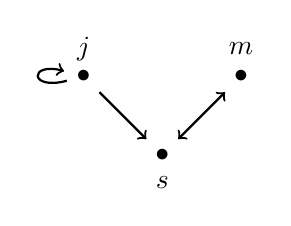
\begin{tikzpicture}

        \node (j) at (0,0)   {$\bullet$};

        \node (m) at (2,0)   {$\bullet$};

        \node (s) at (1,-1)  {$\bullet$};

        \node at (0,0.35)   {$j$};

        \node at (2,0.35)   {$m$};

        \node at (1,-1.35)   {$s$};

        % Arrows
        \path[thick,-to] (j) edge [loop left] (j);
        \draw[->, thick]  (j) -- (s);
        \draw[<->, thick] (m) -- (s);

      \end{tikzpicture}
    \end{center}
  \end{minipage}

\end{frame}

\begin{frame}
  \frametitle{Relations}
  \framesubtitle{Terminology \& notation}

  \begin{itemize}
    \item $R \subseteq X \times Y$ is also called a \textit{binary} relation
    \item if $\tuple{x,y} \in R \subseteq X \times Y$, we can also use
    \begin{itemize}
      \item \textcolor{themecolor}{prefix notation:} $Rxy$ \hfill \mygray{[used in this course; except for math stuff like $1\le2$]}
      \item \textcolor{themecolor}{infix notation:} $xRy$
      \item \textcolor{themecolor}{postfix notation:} $xyR$
    \end{itemize}
    \item domain and range of binary relation $R \subseteq X \times Y$:
          \begin{align*}
            \text{dom}(R) & = \set{x \in X \setbar \text{there is some $y \in Y$ with } Rxy} \\
            \text{range}(R) & = \set{y \in Y \setbar \text{there is some $x \in X$ with } Rxy}
          \end{align*}
  \end{itemize}

\end{frame}

\begin{frame}
  \frametitle{Properties of binary relations}

  \begin{minipage}{0.65\linewidth}
    \begin{small}
      Binary relation $R \subseteq X \times X$ is
      \begin{enumerate}
        \item[] \textit{reflexive} iff $Rxx$ for all $x \in X$
        \item[] \textit{irreflexive} iff $Rxx$ for no $x \in X$
        \item[] \textit{symmetric} iff for all $x,y \in X$ if $Rxy$ then also $Ryx$
        \item[] \textit{asymmetric} iff for no $x,y \in X$ both $Rxy$ and $Ryx$
        \item[] \textit{anti-symmetric} iff for all $x,y \in X$ if $Rxy$ and $Ryx$, then $x = y$
        \item[] \textit{transitive} iff for all $x,y \in X$ if $Rxy$ and $Ryz$, then also $Rxz$
        \item[] \textit{intransitive} iff for all $x,y \in X$ if $Rxy$ and $Ryz$, then not $Rxz$
        \item[] \textit{connected} iff for all $x,y \in X$ either $Rxy$ or $Ryx$ or $x = y$
      \end{enumerate}
    \end{small}
  \end{minipage}
  \hfill
  \begin{minipage}{0.3\linewidth}
    \begin{center}
      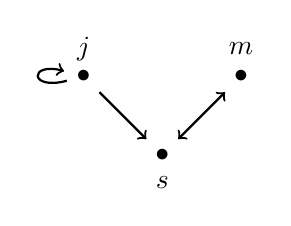
\begin{tikzpicture}

        \node (j) at (0,0)   {$\bullet$};

        \node (m) at (2,0)   {$\bullet$};

        \node (s) at (1,-1)  {$\bullet$};

        \node at (0,0.35)   {$j$};

        \node at (2,0.35)   {$m$};

        \node at (1,-1.35)   {$s$};

        % Arrows
        \path[thick,-to] (j) edge [loop left] (j);
        \draw[->, thick]  (j) -- (s);
        \draw[<->, thick] (m) -- (s);

      \end{tikzpicture}
    \end{center}
  \end{minipage}

\end{frame}


\begin{frame}
  \frametitle{Orders and equivalence relations}
  Binary relation $R \subseteq X \times X$ is said to be:

  \begin{itemize}

    \item  a \textit{partial weak order} iff $R$ is reflexive, anti-symmetric and transitive \\
    \hfill \mygray{[example: relation ``$\subseteq$'' on $\pow{Y}$]}
    \item  a \textit{partial strict order} iff $R$ is irreflexive, asymmetric and transitive \\
    \hfill \mygray{[example: relation ``$\subset$'' on $\pow{Y}$]}
    \item  a \textit{linear weak order} iff $R$ is a partial weak order and connected \\
    \hfill \mygray{[example: relation ``$\le$'' on $\mathds{N}$]}
    \item  a \textit{linear strict order} iff $R$ is a partial strict order and connected \\
    \hfill \mygray{[example: relation ``$<$'' on $\mathds{N}$]}
    \item an \textit{equivalence relation} iff $R$ is reflexive, symmetric and transitive \\
    \hfill \mygray{[example: relation ``has equal cardinality'' on $\pow{Y}$]}

  \end{itemize}

\end{frame}

\end{document}
